\documentclass[8pt]{beamer}\usepackage[]{graphicx}\usepackage[]{color}

\def\expect#1#2{\underset{#1}{\mathbb{E}}\left[#2\right]}
\def\sumn{\sum_{n=1}^N}
\def\x{x}
\def\xvec{X}
\def\w{w}
\def\onevec{1_N}
\def\infl{\psi}

\usetheme{metropolis}           % Use metropolis theme
\usepackage{amsmath}
\usepackage{tikz}


\usepackage{listings}
\lstset
{
    language=[LaTeX]TeX,
    breaklines=true,
    basicstyle=\tt\scriptsize,
    keywordstyle=\color{blue},
    identifierstyle=\color{magenta},
}

\title{TikZ and Beamer for Image Annotation}
\author{Ryan Giordano}
\date{Nov 16th, 2021}
\institute{Massachusetts Institute of Technology}

\begin{document}



%%%%%%%%%%%%%%%%%%%%%%%%%%%%%%%%%%%%%%%%%%%%%%%%%%%%%%%%%%%%%%%%%%%%%%%
%%%%%%%%%%%%%%%%%%%%%%%%%%%%%%%%%%%%%%%%%%%%%%%%%%%%%%%%%%%%%%%%%%%%%%%
%%%%%%%%%%%%%%%%%%%%%%%%%%%%%%%%%%%%%%%%%%%%%%%%%%%%%%%%%%%%%%%%%%%%%%%

\begin{frame}[fragile]{Annotating a graphic using TikZ.}

\begin{center}
\begin{minipage}{0.38\textwidth}
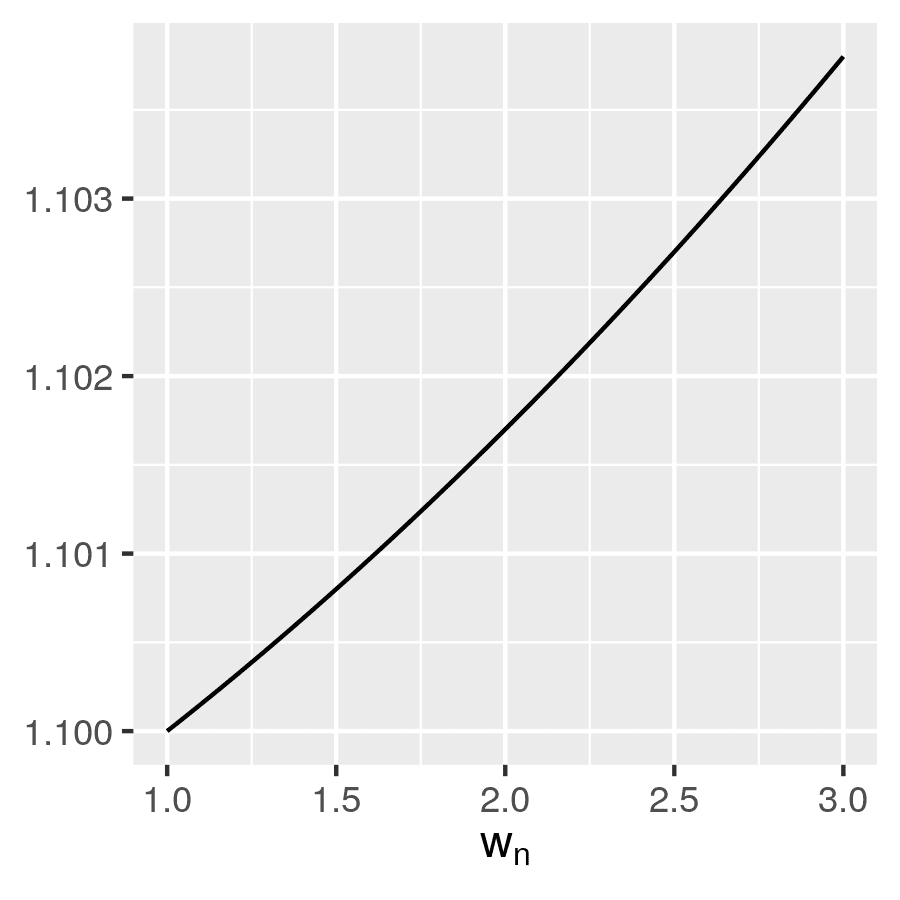
\includegraphics[width=\textwidth]{e_beta_w}
\end{minipage}
\end{center}

%%%%%%%%%%%%%%%%%%%%%%
\hrulefill

Let's annotate this graphic using TikZ.

\begin{lstlisting}
\begin{center}
\begin{minipage}{0.38\textwidth}
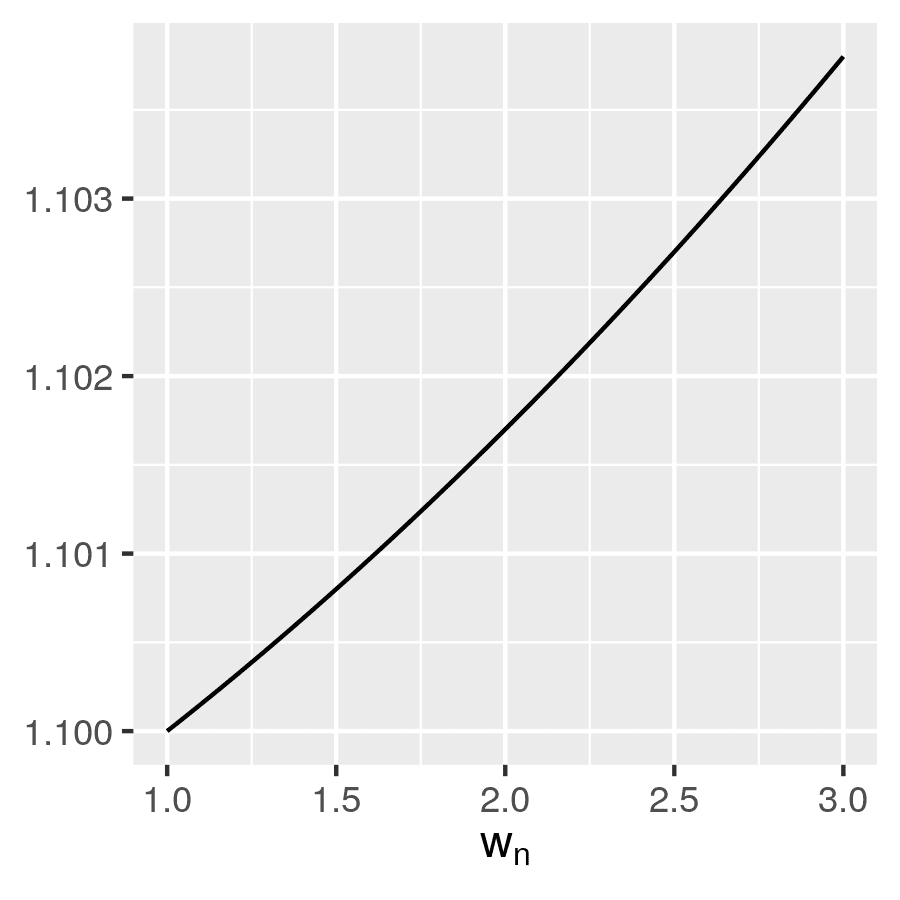
\includegraphics[width=\textwidth]{e_beta_w}
\end{minipage}
\end{center}
\end{lstlisting}

From now on, everything I'm going to do will be within the minipage.

\end{frame}





%%%%%%%%%%%%%%%%%%%%%%%%%%%%%%%%%%%%%%%%%%%%%%%%%%%%%%%%%%%%%%%%%%%%%%%
%%%%%%%%%%%%%%%%%%%%%%%%%%%%%%%%%%%%%%%%%%%%%%%%%%%%%%%%%%%%%%%%%%%%%%%
%%%%%%%%%%%%%%%%%%%%%%%%%%%%%%%%%%%%%%%%%%%%%%%%%%%%%%%%%%%%%%%%%%%%%%%

\begin{frame}[fragile]{How does the IJ work?  Data re-weighting.}

\begin{center}
\begin{minipage}{0.38\textwidth}
    \begin{tikzpicture}
        \node[anchor=south west,inner sep=0] (image) at (0,0) {
            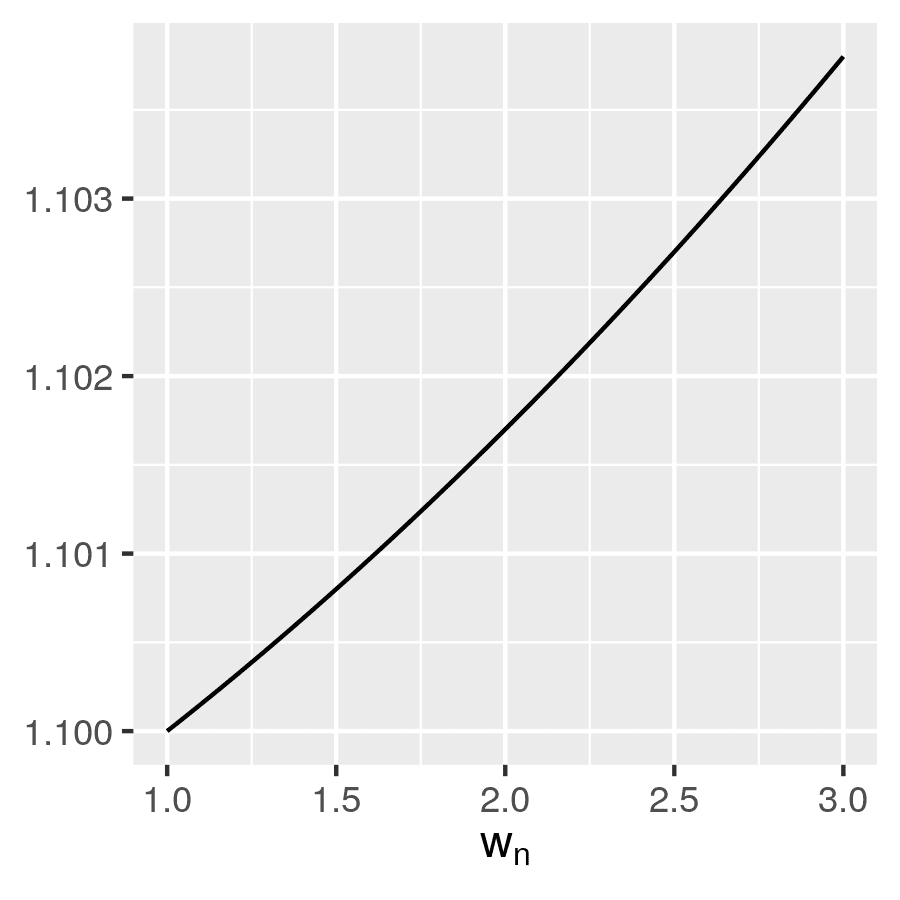
\includegraphics[width=\textwidth]{e_beta_w}
        };
        \begin{scope}[x={(image.south east)},y={(image.north west)}]
            \draw[color=red] (0, 0) circle (0.1);
            \draw[color=green] (1.0, 1.0) circle (0.1);
            \draw[color=blue] (0.1, 0.5) circle (0.1);
            \node[color=red] (hello) at (0.5, 0.5) {HELLO};
        \end{scope}
    \end{tikzpicture}
\end{minipage}
\end{center}

%%%%%%%%%%%%%%%%%%%%%%
\hrulefill

\begin{lstlisting}
\begin{tikzpicture}
    \node[anchor=south west,inner sep=0] (image) at (0,0) {
        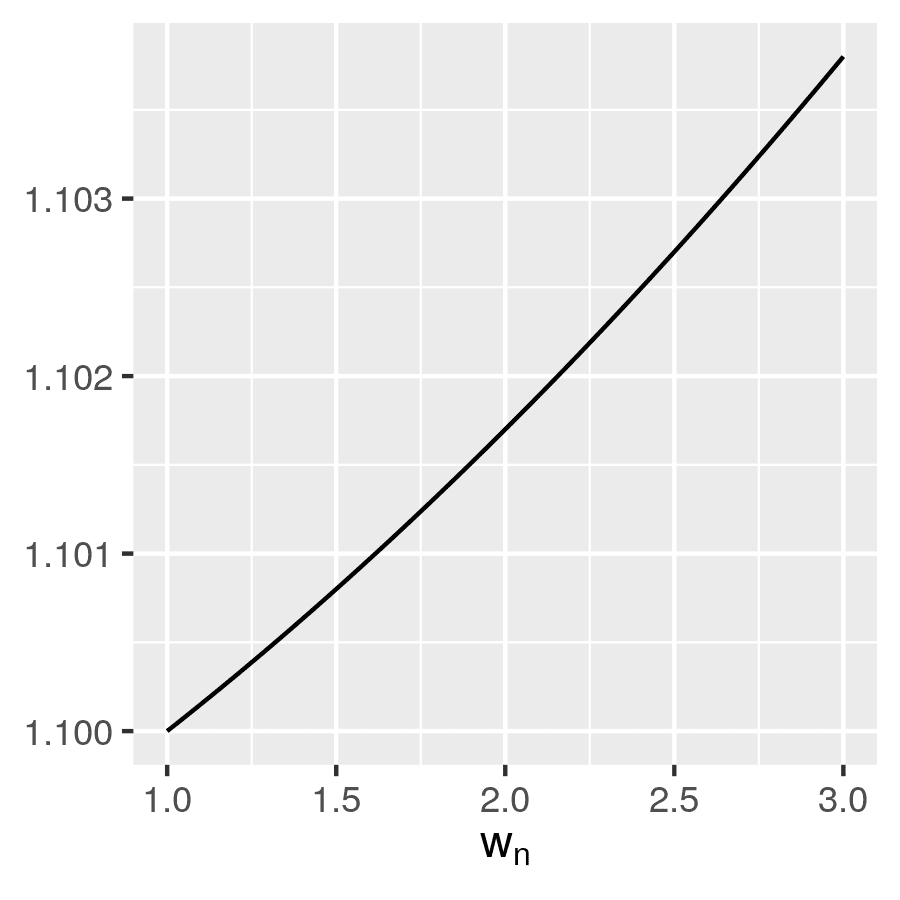
\includegraphics[width=\textwidth]{e_beta_w}
    };
    \begin{scope}[x={(image.south east)},y={(image.north west)}]
        \draw[color=red] (0, 0) circle (0.1);
        \draw[color=green] (1.0, 1.0) circle (0.1);
        \draw[color=blue] (0.1, 0.5) circle (0.1);
        \node[color=red] (hello) at (0.5, 0.5) {HELLO};
    \end{scope}
\end{tikzpicture}
\end{lstlisting}

\end{frame}




%%%%%%%%%%%%%%%%%%%%%%%%%%%%%%%%%%%%%%%%%%%%%%%%%%%%%%%%%%%%%%%%%%%%%%%
%%%%%%%%%%%%%%%%%%%%%%%%%%%%%%%%%%%%%%%%%%%%%%%%%%%%%%%%%%%%%%%%%%%%%%%
%%%%%%%%%%%%%%%%%%%%%%%%%%%%%%%%%%%%%%%%%%%%%%%%%%%%%%%%%%%%%%%%%%%%%%%

\begin{frame}[fragile]{How does the IJ work?  Data re-weighting.}

\begin{center}
\begin{minipage}{0.38\textwidth}
    \begin{tikzpicture}
        \node[anchor=south west,inner sep=0] (image) at (0,0) {
            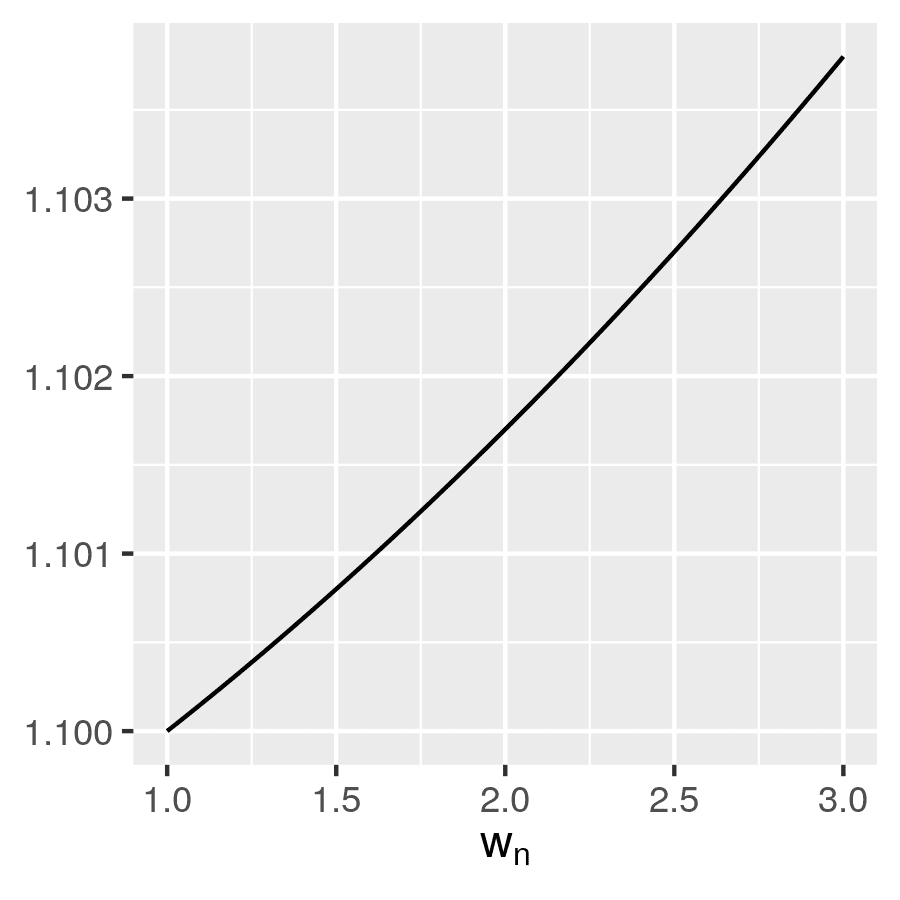
\includegraphics[width=\textwidth]{e_beta_w}
        };
        \begin{scope}[x={(image.south east)},y={(image.north west)}]
            \node[anchor=west, color=red] (y-label) at (0.14, 0.9)
                {$\expect{p(\theta \vert \x, \w)}{\theta}$};
            \node[anchor=east, color=blue] (y-label) at (0.14, 0.9)
                {$\expect{p(\theta \vert \x, \w)}{\theta}$};
        \end{scope}
    \end{tikzpicture}
\end{minipage}
\end{center}

%%%%%%%%%%%%%%%%%%%%%%
\hrulefill

Here and from now on, I'll assume all commands are within the ``scope'' block.

\begin{lstlisting}
\node[anchor=west, color=red] (y-label) at (0.14, 0.9)
    {$\expect{p(\theta \vert \x, \w)}{\theta}$};

\node[anchor=east, color=blue] (y-label) at (0.14, 0.9)
    {$\expect{p(\theta \vert \x, \w)}{\theta}$};
\end{lstlisting}

\end{frame}





%%%%%%%%%%%%%%%%%%%%%%%%%%%%%%%%%%%%%%%%%%%%%%%%%%%%%%%%%%%%%%%%%%%%%%%
%%%%%%%%%%%%%%%%%%%%%%%%%%%%%%%%%%%%%%%%%%%%%%%%%%%%%%%%%%%%%%%%%%%%%%%
%%%%%%%%%%%%%%%%%%%%%%%%%%%%%%%%%%%%%%%%%%%%%%%%%%%%%%%%%%%%%%%%%%%%%%%

\begin{frame}[fragile]{How does the IJ work?  Data re-weighting.}

\begin{center}
\begin{minipage}{0.38\textwidth}
    \begin{tikzpicture}
        \node[anchor=south west,inner sep=0] (image) at (0,0) {
            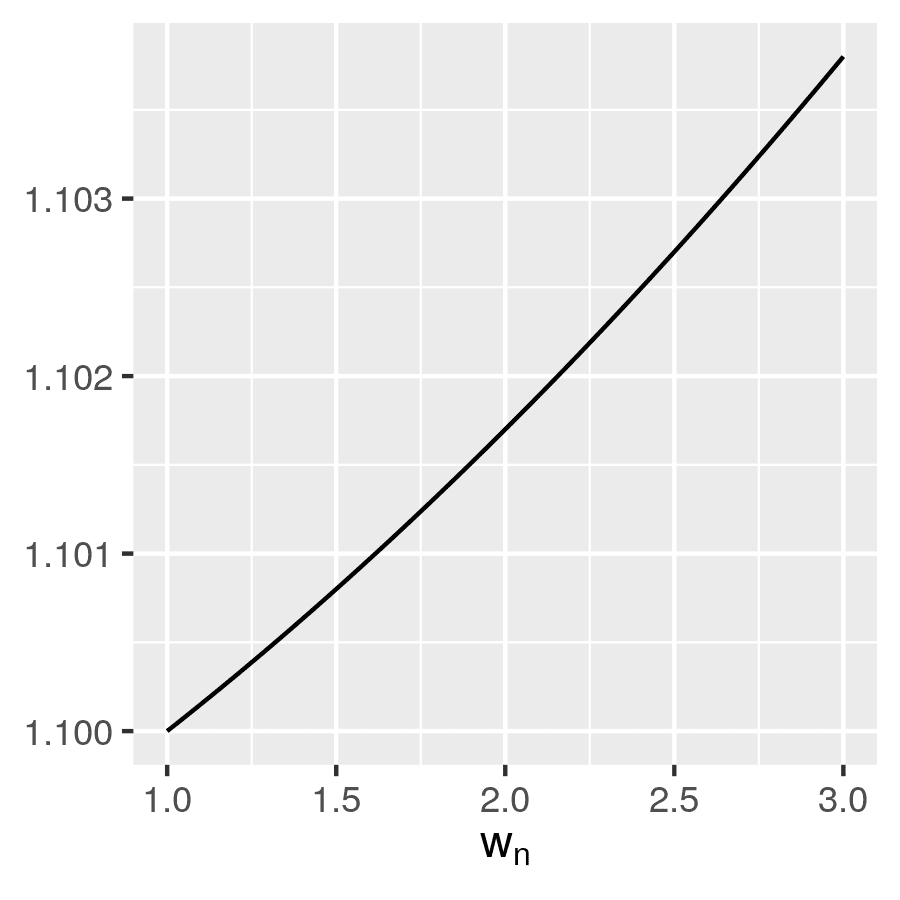
\includegraphics[width=\textwidth]{e_beta_w}
        };
        \begin{scope}[x={(image.south east)},y={(image.north west)}]
            \draw[color=white, fill=white] (-0.2,0) rectangle (0,1);
            \node[anchor=east] (y-label) at (0.14, 0.9)
                {$\expect{p(\theta \vert \x, \w)}{\theta}$};
        \end{scope}
    \end{tikzpicture}
\end{minipage}
\end{center}

%%%%%%%%%%%%%%%%%%%%%%
\hrulefill


\begin{lstlisting}
\draw[color=white, fill=white] (-0.2,0) rectangle (0,1);

\node[anchor=east] (y-label) at (0.14, 0.9)
    {$\expect{p(\theta \vert \x, \w)}{\theta}$};
\end{lstlisting}

\end{frame}



%%%%%%%%%%%%%%%%%%%%%%%%%%%%%%%%%%%%%%%%%%%%%%%%%%%%%%%%%%%%%%%%%%%%%%%
%%%%%%%%%%%%%%%%%%%%%%%%%%%%%%%%%%%%%%%%%%%%%%%%%%%%%%%%%%%%%%%%%%%%%%%
%%%%%%%%%%%%%%%%%%%%%%%%%%%%%%%%%%%%%%%%%%%%%%%%%%%%%%%%%%%%%%%%%%%%%%%

\begin{frame}[fragile]{How does the IJ work?  Data re-weighting.}

\begin{center}
\begin{minipage}{0.38\textwidth}
    \begin{tikzpicture}
        \node[anchor=south west,inner sep=0] (image) at (0,0) {
            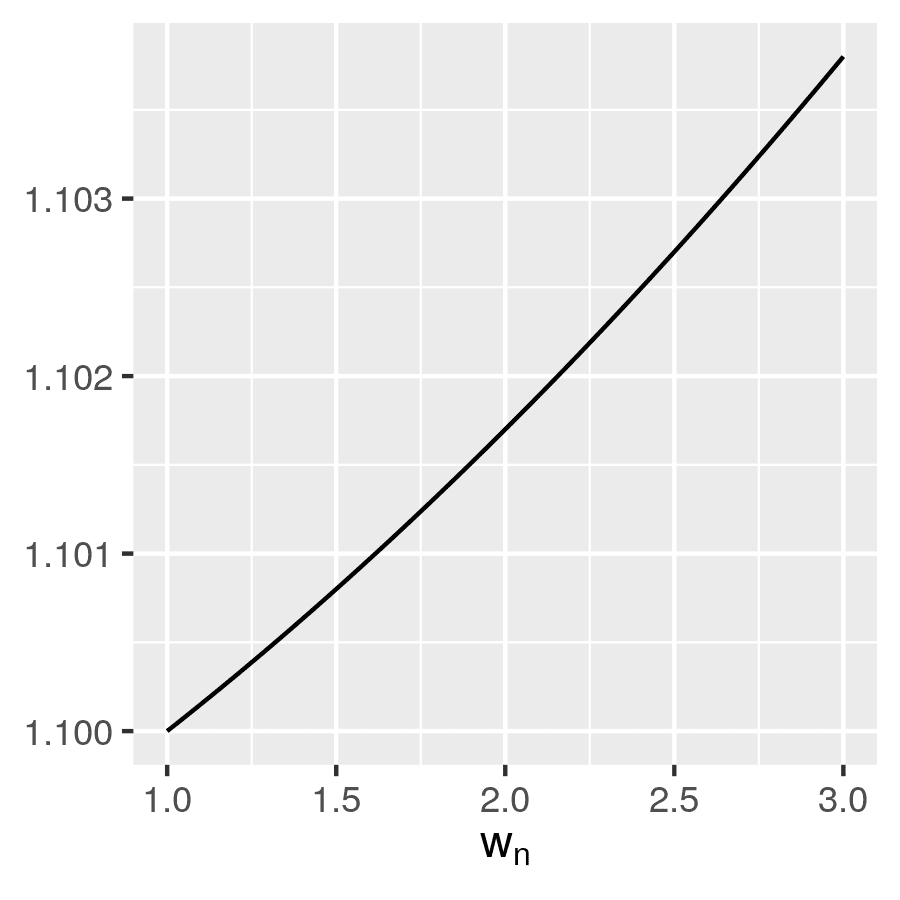
\includegraphics[width=\textwidth]{e_beta_w}
        };
        \begin{scope}[x={(image.south east)},y={(image.north west)}]
            \draw[color=white, fill=white] (-0.2,0) rectangle (0,1);
            \node[anchor=east] (y-label) at (0.14, 0.9)
                {$\expect{p(\theta \vert \x, \w)}{\theta}$};
            \draw[red, thick, -] (0.18,0.18) -- ++(1.2 * 0.6, 1.2 * 0.48);
        \end{scope}
    \end{tikzpicture}
\end{minipage}
\end{center}

%%%%%%%%%%%%%%%%%%%%%%
\hrulefill


\begin{lstlisting}
\draw[red, thick, -] (0.18,0.18) -- ++(1.2 * 0.6, 1.2 * 0.48);
\end{lstlisting}

\end{frame}



%%%%%%%%%%%%%%%%%%%%%%%%%%%%%%%%%%%%%%%%%%%%%%%%%%%%%%%%%%%%%%%%%%%%%%%
%%%%%%%%%%%%%%%%%%%%%%%%%%%%%%%%%%%%%%%%%%%%%%%%%%%%%%%%%%%%%%%%%%%%%%%
%%%%%%%%%%%%%%%%%%%%%%%%%%%%%%%%%%%%%%%%%%%%%%%%%%%%%%%%%%%%%%%%%%%%%%%

\begin{frame}[fragile]{How does the IJ work?  Data re-weighting.}

\begin{center}
\begin{minipage}{0.38\textwidth}
    \begin{tikzpicture}
        \node[anchor=south west,inner sep=0] (image) at (0,0) {
            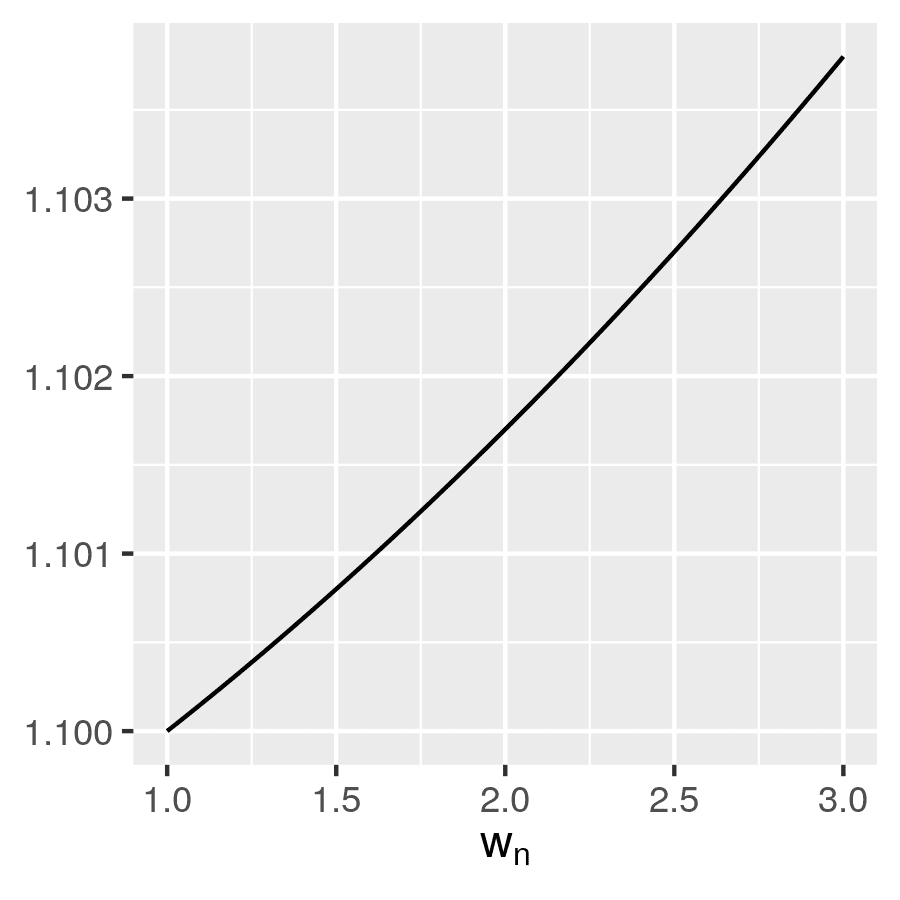
\includegraphics[width=\textwidth]{e_beta_w}
        };
        \begin{scope}[x={(image.south east)},y={(image.north west)}]
            \draw[color=white, fill=white] (-0.2,0) rectangle (0,1);
            \node[anchor=east] (y-label) at (0.14, 0.9)
                {$\expect{p(\theta \vert \x, \w)}{\theta}$};
            \draw[red, thick, -] (0.18,0.18) -- ++(1.2 * 0.6, 1.2 * 0.48);
            \draw[blue, thick, <-] (0.2,0.23) -- ++(0.1,0.25)
                node[above, black, fill opacity=0, text opacity=1]
                {\small $\expect{p(\theta \vert \x)}{\theta}$};
        \end{scope}
    \end{tikzpicture}
\end{minipage}
\end{center}

%%%%%%%%%%%%%%%%%%%%%%
\hrulefill


\begin{lstlisting}
\draw[blue, thick, <-] (0.2,0.23) -- ++(0.1,0.25)
    node[above, black, fill opacity=0, text opacity=1]
    {\small $\expect{p(\theta \vert \x)}{\theta}$};
\end{lstlisting}

\end{frame}




%%%%%%%%%%%%%%%%%%%%%%%%%%%%%%%%%%%%%%%%%%%%%%%%%%%%%%%%%%%%%%%%%%%%%%%
%%%%%%%%%%%%%%%%%%%%%%%%%%%%%%%%%%%%%%%%%%%%%%%%%%%%%%%%%%%%%%%%%%%%%%%
%%%%%%%%%%%%%%%%%%%%%%%%%%%%%%%%%%%%%%%%%%%%%%%%%%%%%%%%%%%%%%%%%%%%%%%

\begin{frame}[fragile]{How does the IJ work?  Data re-weighting.}

\begin{center}
\begin{minipage}{0.38\textwidth}
    \begin{tikzpicture}
        \node[anchor=south west,inner sep=0] (image) at (0,0) {
            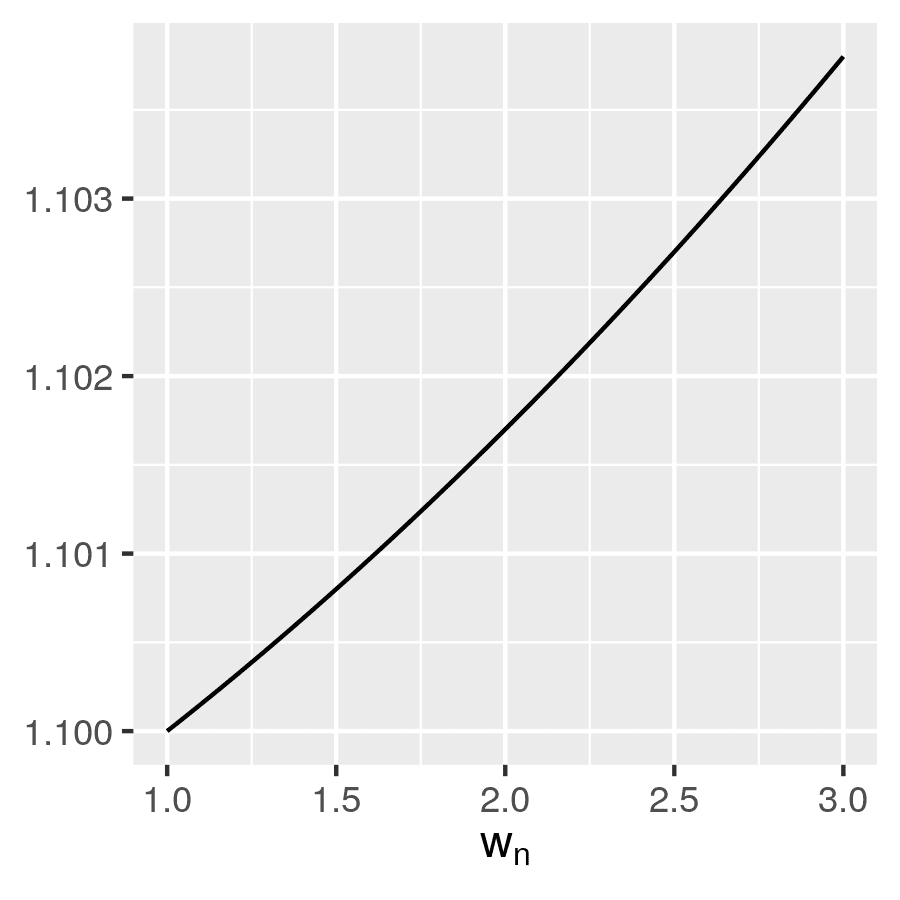
\includegraphics[width=\textwidth]{e_beta_w}
        };
        \begin{scope}[x={(image.south east)},y={(image.north west)}]
            \draw[color=white, fill=white] (-0.2,0) rectangle (0,1);
            \node[anchor=east] (y-label) at (0.14, 0.9)
                {$\expect{p(\theta \vert \x, \w)}{\theta}$};
            \draw[red, thick, -] (0.18,0.18) -- ++(1.2 * 0.6, 1.2 * 0.48);
            \draw[blue, thick, <-] (0.2,0.23) -- ++(0.1,0.25)
                node[above, black, fill opacity=0, text opacity=1]
                {\small $\expect{p(\theta \vert \x)}{\theta}$};
        \end{scope}
    \end{tikzpicture}
\end{minipage}
\end{center}

%%%%%%%%%%%%%%%%%%%%%%
\hrulefill


\begin{lstlisting}
\draw[color=white, fill=white] (-0.2,0) rectangle (0,1);
\node[anchor=east] (y-label) at (0.14, 0.9)
    {$\expect{p(\theta \vert \x, \w)}{\theta}$};
\draw[red, thick, -] (0.18,0.18) -- ++(1.2 * 0.6, 1.2 * 0.48);
\draw[blue, thick, <-] (0.2,0.23) -- ++(0.1,0.25)
    node[above, black, fill opacity=0, text opacity=1]
    {\small $\expect{p(\theta \vert \x)}{\theta}$};
\end{lstlisting}

\end{frame}





%%%%%%%%%%%%%%%%%%%%%%%%%%%%%%%%%%%%%%%%%%%%%%%%%%%%%%%%%%%%%%%%%%%%%%%
%%%%%%%%%%%%%%%%%%%%%%%%%%%%%%%%%%%%%%%%%%%%%%%%%%%%%%%%%%%%%%%%%%%%%%%
%%%%%%%%%%%%%%%%%%%%%%%%%%%%%%%%%%%%%%%%%%%%%%%%%%%%%%%%%%%%%%%%%%%%%%%

\begin{frame}[fragile]{How does the IJ work?  Data re-weighting.}

\begin{center}
\begin{minipage}{0.38\textwidth}
    \begin{tikzpicture}
        \node[anchor=south west,inner sep=0] (image) at (0,0) {
            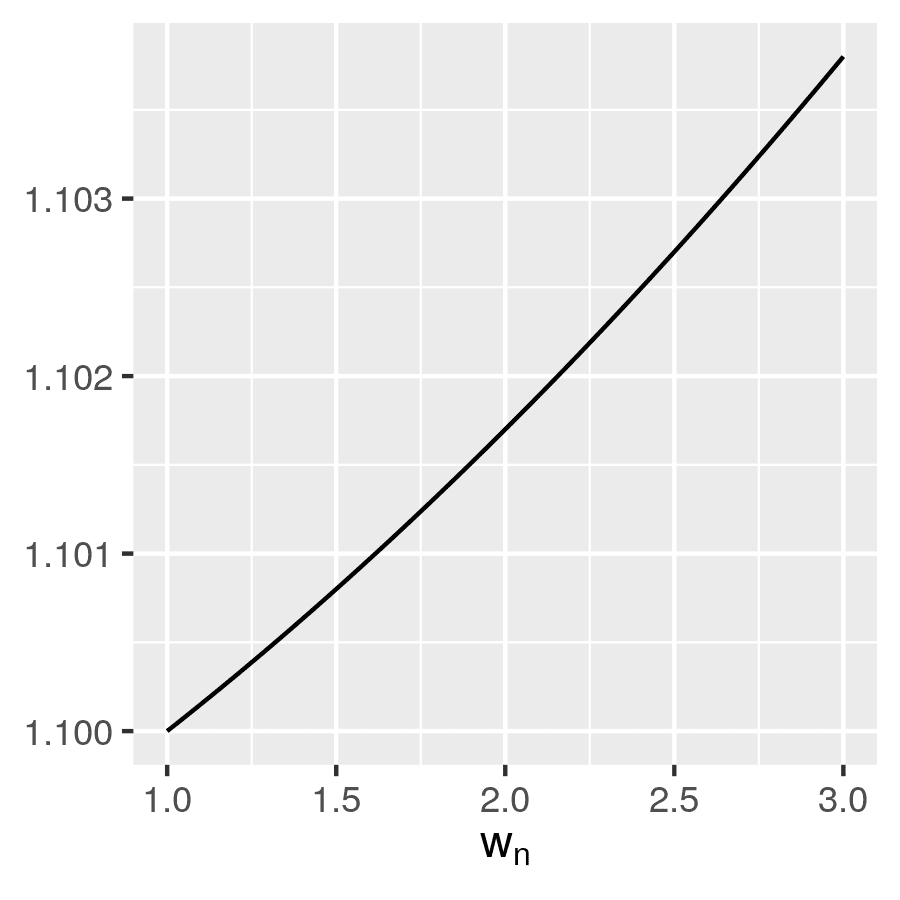
\includegraphics[width=\textwidth]{e_beta_w}
        };
        \begin{scope}[x={(image.south east)},y={(image.north west)}]
            \draw[color=white, fill=white] (-0.2,0) rectangle (0,1);
            \node[anchor=east] (y-label) at (0.14, 0.9)
                {$\expect{p(\theta \vert \x, \w)}{\theta}$};
            \onslide<2->{
                \draw[red, thick, -] (0.18,0.18) -- ++(1.2 * 0.6, 1.2 * 0.48);
            }
            \onslide<3->{
                \draw[blue, thick, <-] (0.2,0.23) -- ++(0.1,0.25)
                    node[above, black, fill opacity=0, text opacity=1]
                    {\small $\expect{p(\theta \vert \x)}{\theta}$};
            }
        \end{scope}
    \end{tikzpicture}
\end{minipage}
\end{center}

%%%%%%%%%%%%%%%%%%%%%%
\hrulefill


\begin{lstlisting}
\draw[color=white, fill=white] (-0.2,0) rectangle (0,1);
\node[anchor=east] (y-label) at (0.14, 0.9)
    {$\expect{p(\theta \vert \x, \w)}{\theta}$};
\onslide<2->{
    \draw[red, thick, -] (0.18,0.18) -- ++(1.2 * 0.6, 1.2 * 0.48);
}
\onslide<3->{
    \draw[blue, thick, <-] (0.2,0.23) -- ++(0.1,0.25)
        node[above, black, fill opacity=0, text opacity=1]
        {\small $\expect{p(\theta \vert \x)}{\theta}$};
}
\end{lstlisting}

\end{frame}




%%%%%%%%%%%%%%%%%%%%%%%%%%%%%%%%%%%%%%%%%%%%%%%%%%%%%%%%%%%%%%%%%%%%%%%
%%%%%%%%%%%%%%%%%%%%%%%%%%%%%%%%%%%%%%%%%%%%%%%%%%%%%%%%%%%%%%%%%%%%%%%
%%%%%%%%%%%%%%%%%%%%%%%%%%%%%%%%%%%%%%%%%%%%%%%%%%%%%%%%%%%%%%%%%%%%%%%

\begin{frame}{Further reading}

Beamer:
{\tiny
% \url{https://www.overleaf.com/learn/latex/Beamer_Presentations%3A_A_Tutorial_for_Beginners_(Part_1)%E2%80%94Getting_Started}\\
\begin{itemize}
\item Google ``beamer tutorial''
\item \url{https://warwick.ac.uk/fac/sci/physics/research/cfsa/people/pastmembers/wuensch/workshoplatex/beamertutorialkwuensch.pdf}
\item \url{https://www.texdev.net/2014/01/17/the-beamer-slide-overlay-concept/}\\
\end{itemize}
}

TikZ:
{\tiny
\begin{itemize}
\item \url{https://www.overleaf.com/learn/latex/TikZ_package}
\item \url{https://www.math.uni-leipzig.de/~hellmund/LaTeX/pgf-tut.pdf}
\item \url{https://latexdraw.com/how-to-annotate-an-image-in-latex/}
\item \url{https://tex.stackexchange.com/questions/9559/drawing-on-an-image-with-tikz}
\end{itemize}
}

\end{frame}


\end{document}
